\section{3D Printing Toolchain}

\subsection{Extruder}

\indent

The extruder is the mechanism responsible for depositing the filament in a 3D printing system. Generally, this mechanism includes a motor that drives a gripping mechanism, which reels in and pushes the filament into a heated nozzle. The nozzle heats the filament into a \emph{mushy} state and lays the filament on the printing bed or on an already printed layer to create the part.\\

In the case of our carbon fiber 3D printer, the extruder is required to mount to the robot arm, be compact\footnote{The compact size is required for two reasons. First, to ensure that induced torque on the robot arm joints and gripper remain within safe operating conditions. Second, to readily permit the nozzle to deposit material when not perpendicular to the build platform, which will be required for printing curved layers.}, and accept filaments of a variety of sizes (likely ranging in diameter from 1.75 mm to 3 mm).  

\begin{figure}[htp]
\centering
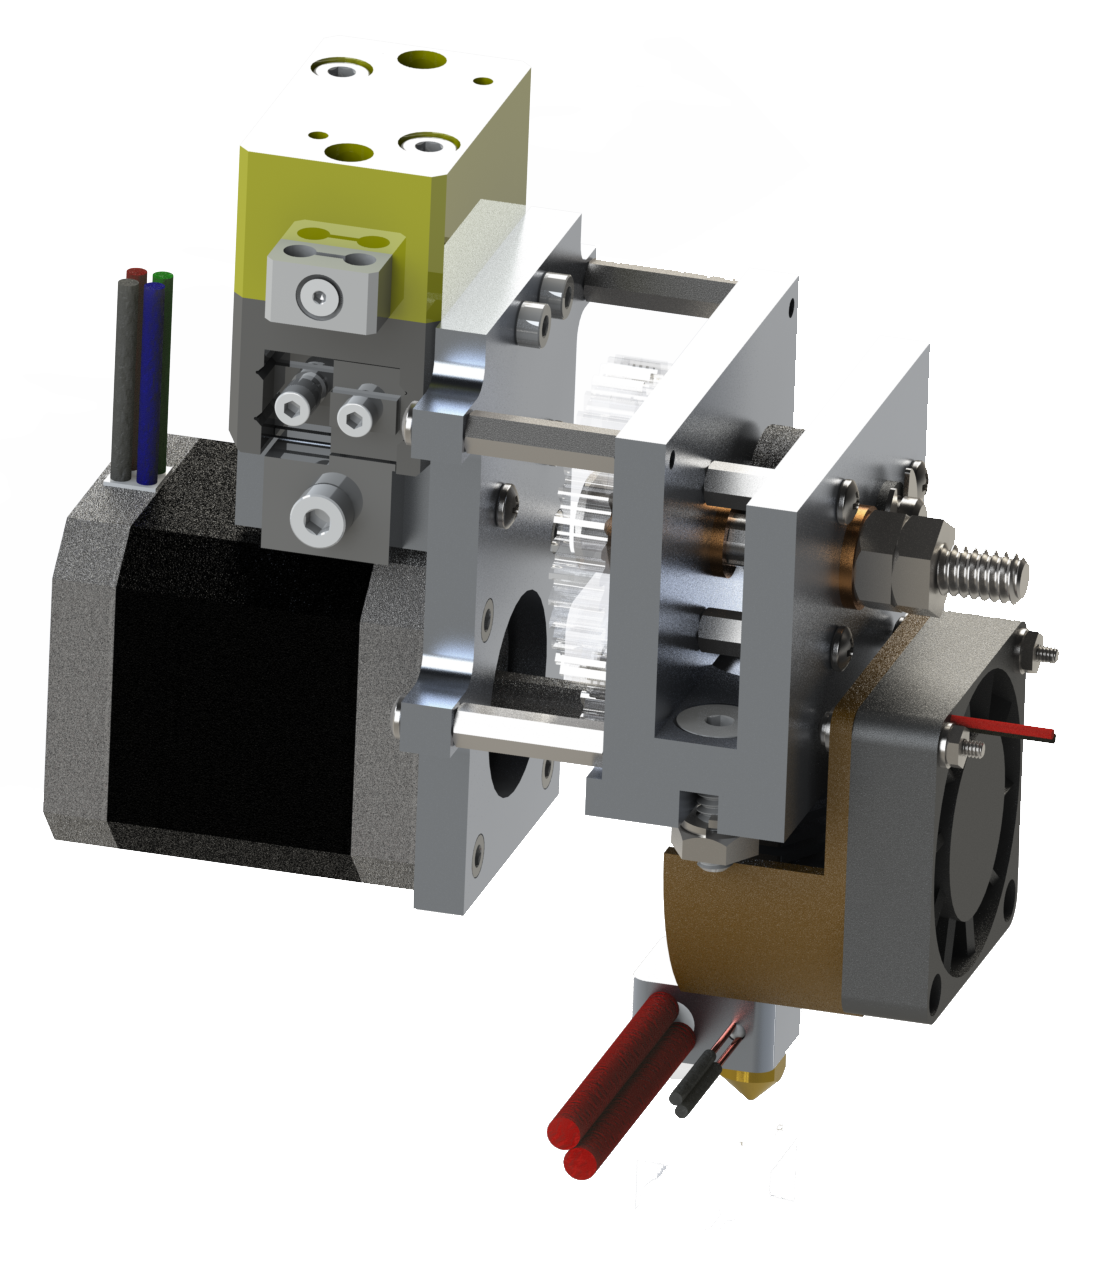
\includegraphics[width=0.5\textwidth]{./figures/extruder-iso}
\caption{An isometric render of the final extruder design.}
\label{fig:flowchart}
\end{figure}

\begin{figure}[htp]
\centering
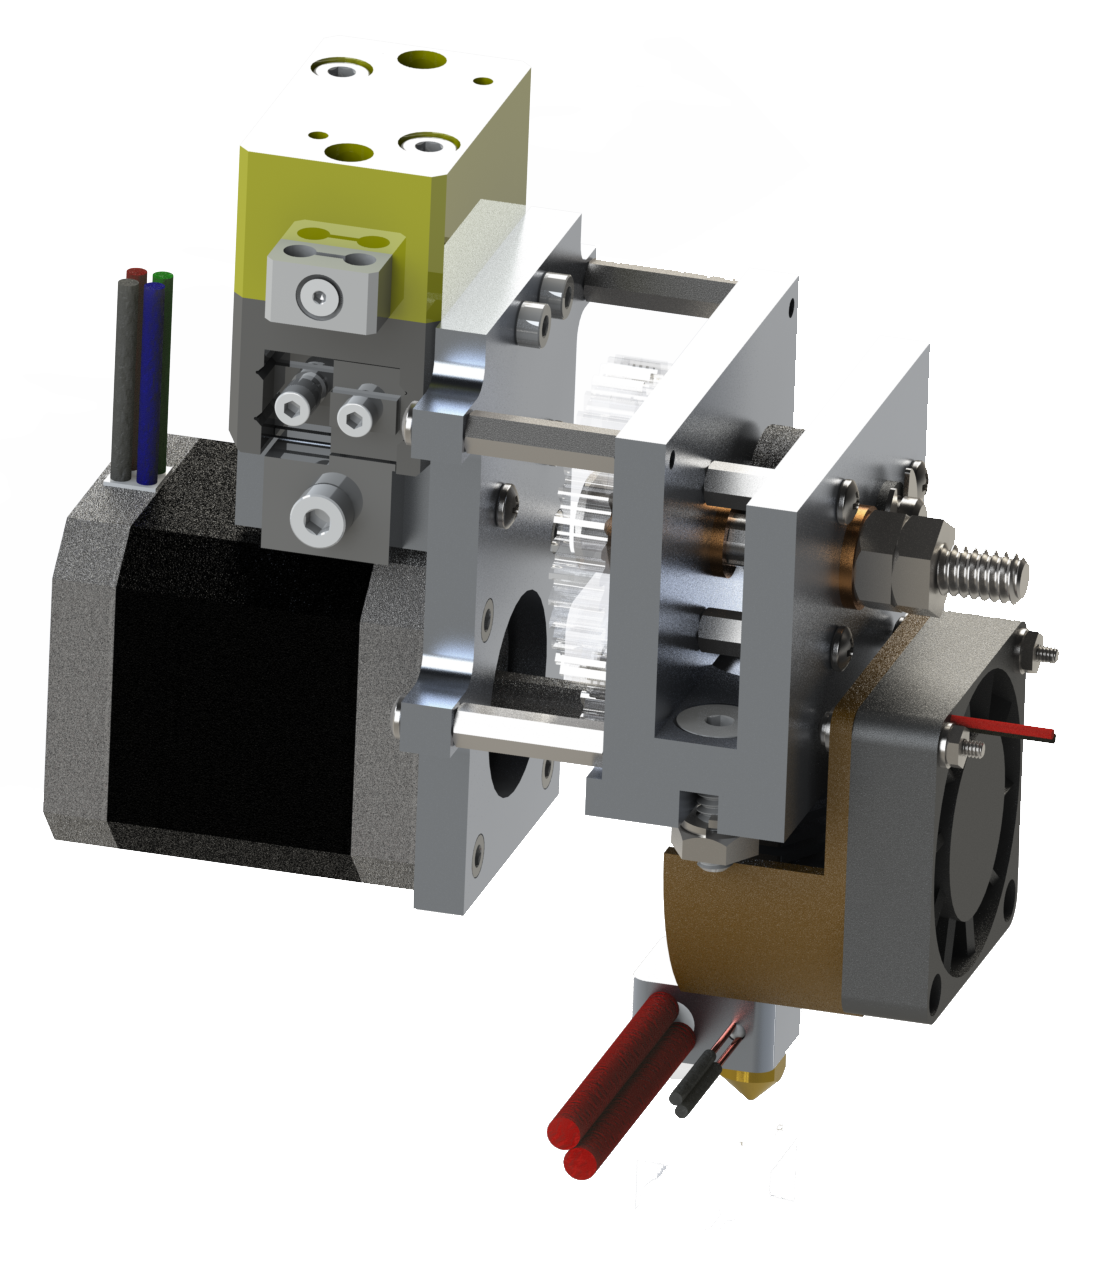
\includegraphics[width=0.5\textwidth]{./figures/extruder-iso}
\caption{An isometric render of the final extruder design.}
\label{fig:flowchart}
\end{figure}

\begin{figure}[htp]
\centering
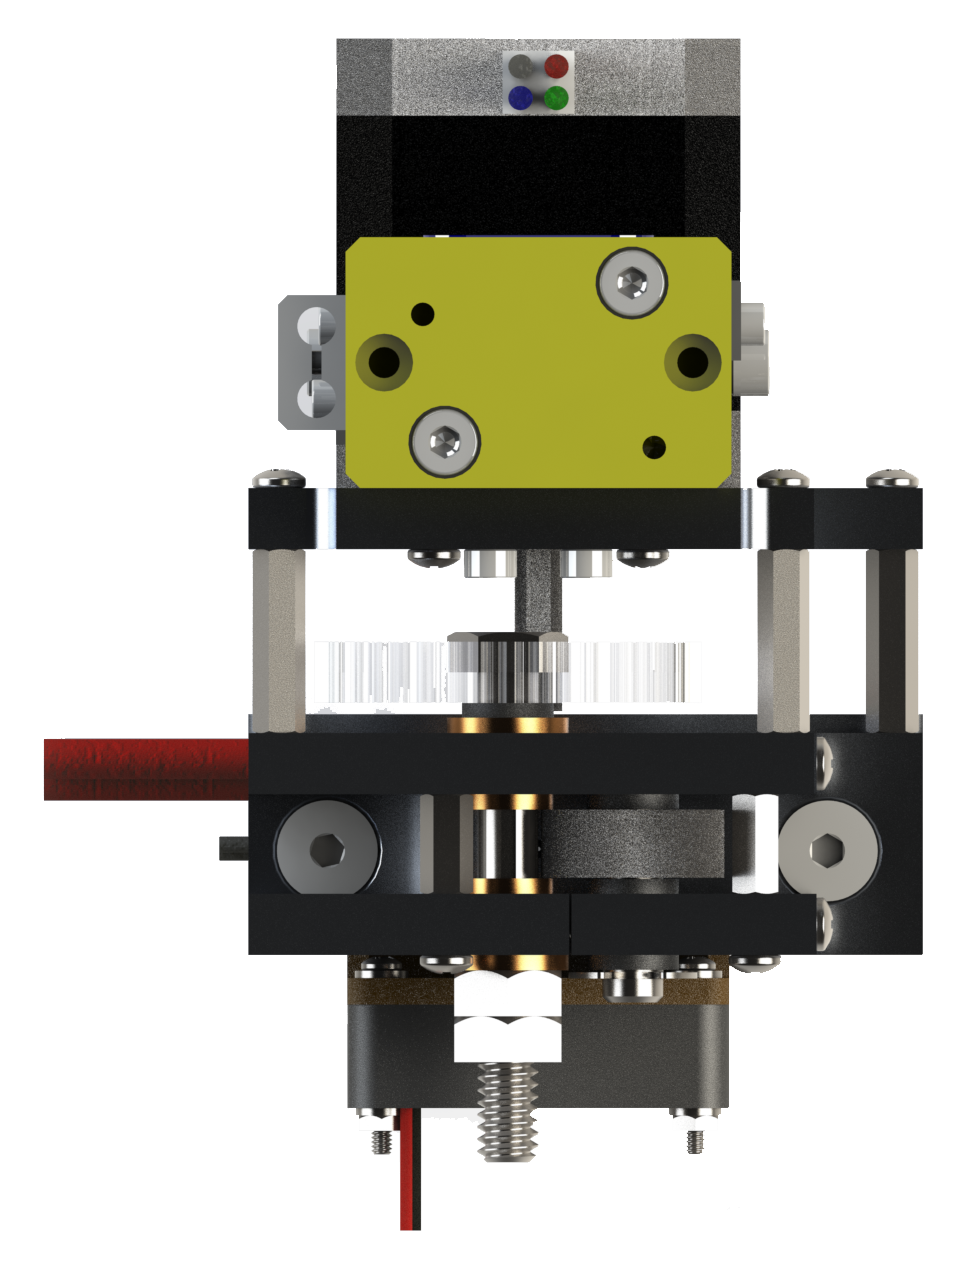
\includegraphics[width=0.5\textwidth]{./figures/extruder-top}
\caption{A front view render of the final extruder design.}
\label{fig:flowchart}
\end{figure}

\begin{figure}[htp]
\centering
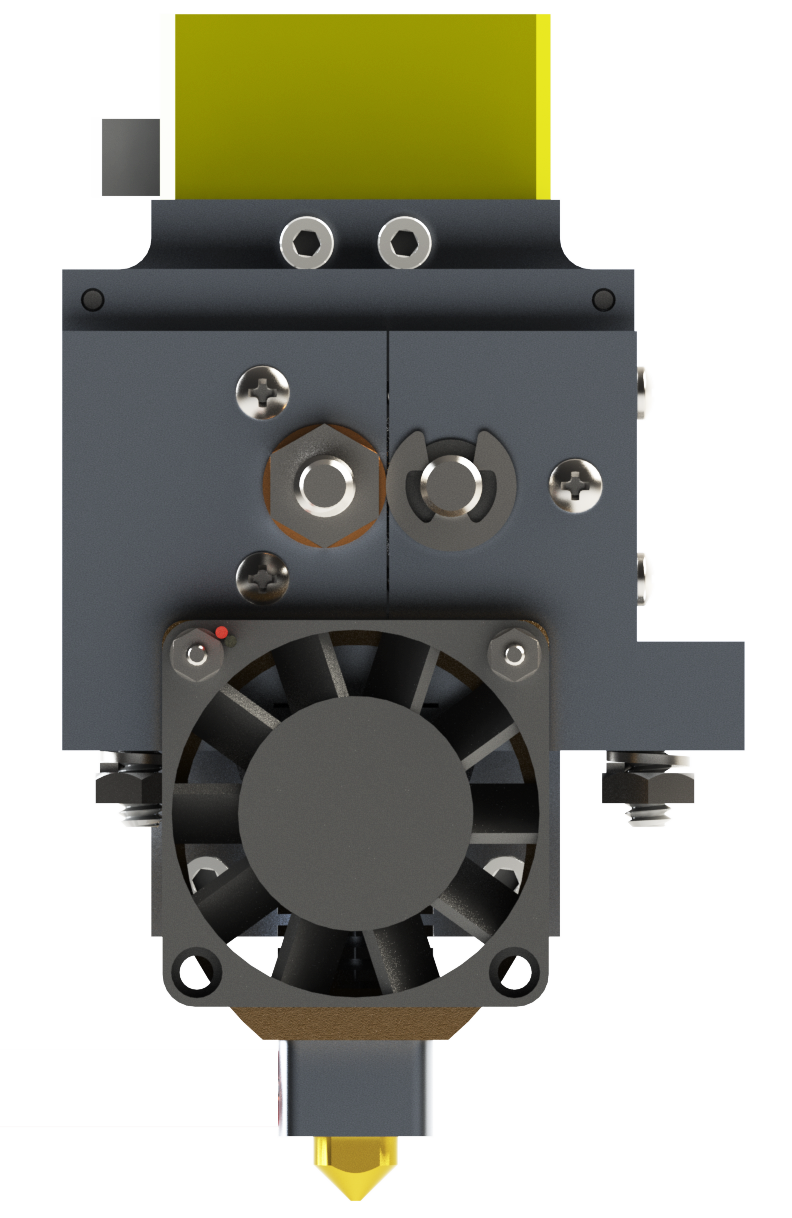
\includegraphics[width=0.5\textwidth]{./figures/extruder-front}
\caption{A top view render of the final extruder design.}
\label{fig:flowchart}
\end{figure}

\clearpage

\subsection{Control Electronics}
\indent 

The extruder is controlled by a Megatronics control board, which was developed for the RepRap open source 3D printer project. The board contains all the necessary electronics to drive a Cartesian coordinate based FDM desktop 3D printer. The board can drive numerous positioning and extruder motors, heating elements, sensors, displays, and more. Because the FANUC robot handles the extruder positioning, the Megatronics board will be used to control the extruder elements only. 

When used in RepRap printers, the Megatronics board is typically used with one of several open source firmwares that are also associated with the RepRap project. Because these firmwares were designed with Cartesian desktop FDM printers in mind, they work well with the Megatronics board. The chosen firmware is uploaded to the board using a USB cable. For the FANUC-mounted extruder, a suitable firmware will be chosen and modified to work with the FANUC robot.

The firmware will be modified to control only the components present on the FANUC-mounted extruder. The firmware's timing functions must be modified as well. Normally, the firmware calculates its own filament feed rates and motor speeds. Because the FANUC controller is much less flexible than the RepRap firmware, the firmware will be modified to monitor the FANUC robot speed and position, and act accordingly. 

\subsection{Slicing Algorithm and Layer Generation}

\indent



sample text
